\section{Transdução inter-corpora}
\label{sec:treino_metodologia}

Neste trabalho, deseja-se a transdução entre um \textit{corpus} em dado formato X, noutro num formato Y, de modo que não haja perda lexical, ou seja, sem afetar as palavras presentes no \textit{corpus} original. Podemos considerar, portanto, o transdutor como uma função
\footnote{Para um debate mais aprofundado sobre o embasamento matemático de transdutores, recomenda-se a leitura de \cite{weightedTransducersMohri}}
equivalente à \ref{eq:funcao_transdutor}:
\begin{center}
    \begin{equation}
\label{eq:funcao_transdutor}
    t(S) = S', dado\;S = CO, S' \in CD.
\end{equation}
\end{center}

Sendo CD o \textit{Corpus} de Origem (CO), a converter, e (CD) o Corpus de Destino, a ser convertido.

O procedimento de transdução consiste de 4 etapas principais: 
\begin{enumerate}
    \item Escolha dos \textit{corpora}; 
    \item Estudo das estruturas do CO e do CD;
    \item Planejamento de equivalências;
    \item Construção do transdutor
\end{enumerate}

\begin{center}
    \begin{figure}[!ht]
    \centering
    % \includegraphics{}
    \includesvg[width=.8\textwidth]{imagens/fluxograma_metodologia}
    % \includesvg{imagens/cintil_pcfg}
    \caption[Fluxograma descrevendo a metodologia inter-\textit{corpora}]{Fluxograma descrevendo a metodologia inter-\textit{corpora}}
    \label{fig:fluxograma_metodologia}
\end{figure}
\end{center}

\subsection{Escolha dos \textit{corpora}}
\label{subsec:escolha_corpora}

A escolha dos \textit{corpora} pode parecer um procedimento trivial, num primeiro momento, mas pode fazer com que o construtor de transdutores deixe de analisar coisas importantes. 

Primeiramente, é preciso saber qual será a finalidade da transdução. No caso deste trabalho, o objetivo na construção do transdutor é fazer o treinamento de um \textit{parser} escolhido. Dado esse ponto de partida, a conversão inter-\textit{corpora} não pode perder informação lexical, ou seja, não serão alteradas as palavras e suas estruturas. Também, é importante que as estruturas internas do produto da transdução sejam análogos ao do \textit{corpus} de destino.

No contexto deste trabalho, a escolha do CD foi ocasionada pela necessidade: desejava-se utilizar o Stanford Parser para análise, e este \textit{parser} está adaptado a entradas no formato Penn Treebank. Portanto, nosso CD é o PTB. 

Os CO demandaram mais pesquisa. Fez-se necessário que, primeiramente, fossem \textit{corpora} da língua portuguesa, principalmente das variantes brasileira e europeia. Também, para facilitar o procedimento de transdução, deu-se preferência à \textit{corpora} cujo formato se assemelhasse ao do PTB. Por fim, é necessário que exista uma documentação bem desenvolvida, tanto de CO como de CD, pois com base nelas serão feitas as próximas etapas.

Nesse sentido, optar por CINTIL e BOSQUE fica mais evidente. O CINTIL possui estruturas internas semelhantes às do PTB, além de um \textit{tagset} mais simplificado. Também, possui um número grande (10.140) de sentenças classificadas. O BOSQUE, por sua vez, possui uma documentação melhor resolvida (pelas análises realizadas neste trabalho), um \textit{tagset} expressivo (com menos redundâncias), e está disponível gratuitamente.

\subsection{Estudo das estruturas do CO e do CD}
\label{subsec:estruturas_corpora}

O estudo das estruturas internas dos \textit{corpora} é peça chave na transdução inter-\textit{corpora}. É fundamental saber como as sentenças em cada \textit{corpus} se estrutura. Existe um ponto ainda mais fundamental: Sabendo-se que os \textit{corpora} são, em resumo, conjuntos de dados em forma de texto, qual o formato do arquivo a ser lido para ser transduzido? Como tal arquivo é escrito? O que o transdutor deve considerar ou ignorar em cada análise? Para utilizar o BOSQUE como exemplo, foi utilizado o formato de arquivo que emulava o PTB, portanto eram feitas as separações (bracketing) com o uso de parênteses. Porém, se fosse utilizado o formato original, estilo Árvores Deitadas (AD, ver sessão \ref{subsubsec:florestasintatica}), seria necessário considerar os símbolos de $=$ no processo de reconstrução da estrutura de árvore. O transdutor construído corre a sequencia de caracteres procurando por símbolos \textquote{abre parênteses} para iniciar a construção de uma nova sub-árvore, e o seu par \textquote{fecha parênteses} para concluir a reconstrução da mesma sub-árvore. Se fosse utilizado o arquivo em AD, seria necessária outra estratégia de reconstrução \textquote{arbórea}. Por exemplo, poderia-se contar a quantidade de \textquote{=} no começo de cada linha e, se a quantidade aumenta, implicaria num novo nível da árvore; a redução implicaria no final da sub-árvore.

Deve-se dar atenção, também, ao \textit{tagset} de cada \textit{corpora}. Este tópico será mais explorado na sessão \ref{subsubsec:tags_correlacionadas}, mas deve-se ter em mente: quais as \textit{tags} que cada \textit{corpus} possui? Quais semelhanças e diferenças?

Por fim, faz-se necessário o estudo de estruturas internas. Como será visto com detalhes em \ref{sec:treinando_sp_cintil} e \ref{sec:treinando_sp_bosque}, diversos arranjos internos exigem uma adaptação específica, e é importante tê-las em mente ao desenvolver o transdutor. Porém, a experiência da prática demonstra que muitas vezes, o \textit{parser} que apontará tais estruturas para o desenvolvedor, quando houver erros de execução durante os treinamentos.

\subsection{Planejamento das equivalências}
\label{subsec:planejamento_equivalencias}

Esta etapa está intrinsecamente ligada à etapa anterior (\ref{subsec:estruturas_corpora}). Aqui, serão planejadas as conversões propriamente ditas. O Planejamento de Equivalências pode ser subdividido em 3 categorias principais:
\begin{enumerate}
    \item Identificação de \textit{tags} correlacionadas
    \item Identificação de \textit{tags} conceitualmente semelhantes
    \item Identificação de \textit{tags} que exigem modificações estruturais
\end{enumerate}
O desenvolvedor deve criar uma tabela de equivalências, onde de um lado estarão as \textit{tags} do CO, e do outro, as \textit{tags} do CD. A coluna de  \textit{tags} do CO será preenchida a cada uma das etapas acima. Exemplos destas tabelas podem ser vistos nas Sessões \ref{sec:treinando_sp_cintil} e \ref{sec:treinando_sp_bosque}.

\subsubsection{Identificação de \textit{tags} correlacionadas}
\label{subsubsec:tags_correlacionadas}

Nesta etapa, serão identificadas as \textit{tags} que podem ser transduzidas diretamente do CO para o CD, sem perda de significado. Tais \textit{tags}, em geral, não possuem grande dificuldade de identificação: a tradução dos seus nomes já costuma ser esse indicativo. Por exemplo: Para o CINTIL, como demonstrado na Tabela \ref{tab:cintil_tags} da Sessão \ref{sec:treinando_sp_cintil}, a leitura de seu manual \cite[p~4]{cintil_handbook} aponta que \textquote{\textit{adjectives}} recebem a \textit{tag} $A$. O Manual de Marcação do Penn Treebank \cite[p~1]{posPTBguidelines}, por sua vez, define \textquote{\textit{adjectives}} como $JJ$. A tabela de correlações pode, portanto, ser preenchida com a correlação $A / JJ$. O BOSQUE define suas \textit{tags} em português. Nestes casos uma tradução simples resolverá a questão: Se por um lado o BOSQUE não tem uma tag para \textquote{adjectives}, por outro existe a tag \textquote{adjectivos}. Portanto, na tabela de correlações BOSQUE/PTB, será preenchida a linha $adj / JJ$.

\subsubsection{Identificação de \textit{tags} conceitualmente semelhantes}
\label{subsubsec:tags_conceit_semelhantes}

Existem \textit{tags} que, apesar de sua nomenclatura não indicar uma conversão direta, uma análise de definição pode apontar o caminho correto. Por exemplo, o \textit{tagset} do BOSQUE, possui a \textit{tag} $fcl$, que é definida por \textquote{Forma Oracional Finita}. O \textit{tagset} do PTB não possui algo semelhante. A definição de $fcl$ em \cite[p~12]{afonso2006arvores} informa que:

\begin{quote}
    \textquote{A oração finita (fcl) contém um verbo de forma finita. [\ldots] A estrutura interna das orações finitas e não-finitas inclui um predicador (P) e argumentos ou adjuntos verbais.} 
\end{quote}

Tal estrutura pode ser classificada como um Sintagma Verbal. E, por \cite[p~321]{buildingPTB}, tal sintagma é marcado por $VP$. Assim, a tabela recebe a linha $fcl / VP$.

\subsubsection{Identificação de \textit{tags} que exigem modificações estruturais}
\label{subsubsec:tags_mudancas_estruturais}

Por fim, o modelo de \textit{tags} que demandam mais trabalho de pesquisa e adaptação são aquelas que não permitem transduções diretas. Um exemplo marcante são as \textit{tags} de coordenação de ambos os CO escolhidos, $CONJP$ para o CINTIL e $CU$ para o BOSQUE. Ambas serão abordadas em suas respectivas sessões, \ref{subsec:cintil-conj} e \ref{subsec:cu}.

Nestes casos, faz-se necessária, em primeiro lugar, o entendimento do que tal estrutura representa gramaticalmente na linguagem. O livro base para este trabalho foi \cite{Castilho2010gramatica}, e nele foram baseadas a maior parte das pesquisas teóricas sobre linguagem e gramática. Também foi bastante utilizado \cite{mioto2013novo}, para dúvidas linguísticas e estruturais. Em seguida, é necessário o estudo e domínio da forma como tal estrutura é descrita / implementada no CO, e no CD.

\subsection{Construção do Transdutor}
\label{subsec:construcao_transdutor}
Neste trabalho, o transdutor $t(x)$ é um algoritmo de Busca em Profundidade, que varre a cadeia de caracteres de entrada S, $S = [w_1w_2\ldots w_n],\; w_i \in \Sigma^*,S \in CO$ e tem como objetivo converter tal cadeia na cadeia S', $S'\in CD$. Sendo CO uma sequencia de sentenças S, $CO=[S_1,S_2,\ldots,S_n]$, ao final de $t(S)=S'$, será gerado um conjunto de S' de estrutura análoga às do CD, [$S_1,S_2',\ldots,S_n']\in CD$. 

No primeiro momento do transdutor, as cadeias de entrada são percorridas apenas uma vez por iteração da recursão. Nesta varredura, a estrutura de árvore é construída. A cada marcador de começo de sub-árvore $w_i$ (\textquote{abre parênteses}, em ambas COs do trabalho), inicia uma nova iteração recursiva, baseada numa nova sub-cadeia $S_{i+1,j},\;i<j,\;0\leq i,\; j\leq n$. Nesta nova interação, o procedimento se repete até encontrar o simbolo de final de sub-árvore $w_j$ (\textquote{fecha parênteses} em ambos os COs). Nesse momento, a varredura de sub-árvore se encerra, a estrutura de dados é atualizada com essa sub-árvore, e a varredura continua a partir de $w_{i+1}$.

Durante a varredura por sub-árvore / nó, são identificadas as \textit{POS tags}. Em ambos COs, as POS, se localizam logo após \textquote{(} (particularidades serão pormenorizadas nas Sessões \ref{sec:treinando_sp_cintil} e \ref{sec:treinando_sp_bosque}). Cadeias de caracteres anteriores ao \textquote{)} são considerados palavras, ou seja $S_{i,j}=[(, w^*,\;,w^*,)],\;w\in \Sigma$ indica um nó. Ao identificar uma \textit{tag}, o nó lógico recebera essa \textit{tag}. Palavras não são modificadas. \textit{Tags} identificadas como \textquote{problemáticas}, ou seja, \textit{tags} da categoria 3, recebem uma marca específica.

Na segunda etapa, as operações ocorrem diretamente na estrutura de dados gerada. É aqui que as \textit{tags} são transduzidas, caso sejam das categorias 1 e 2. \textit{Tags} da categoria 3, que foram marcadas, serão resolvidas. 
Existem pormenores sobre a detecção e adaptação de sinais gráficos (ponto, por exemplo), também.
Sua descrição será feita nas sessões \ref{sec:treinando_sp_cintil} e \ref{sec:treinando_sp_bosque}. Recomenda-se a leitura do algoritmo desenvolvido.

Por fim, na terceira etapa, é feita a impressão textual da estrutura de dados de modo análogo ao formato do CD. É feita uma nova Busca em Profundidade, gerando a cadeia de caracteres final. Poucas adaptações precisam ser feitas nesse momento.

A Figura \ref{fig:fluxograma_transdutor} demonstra as etapas realizadas pelo transdutor.

\begin{center}
    \begin{figure}[!ht]
    \centering
    % \includesvg[width=\textwidth]{imagens/fluxograma_transdutor}
    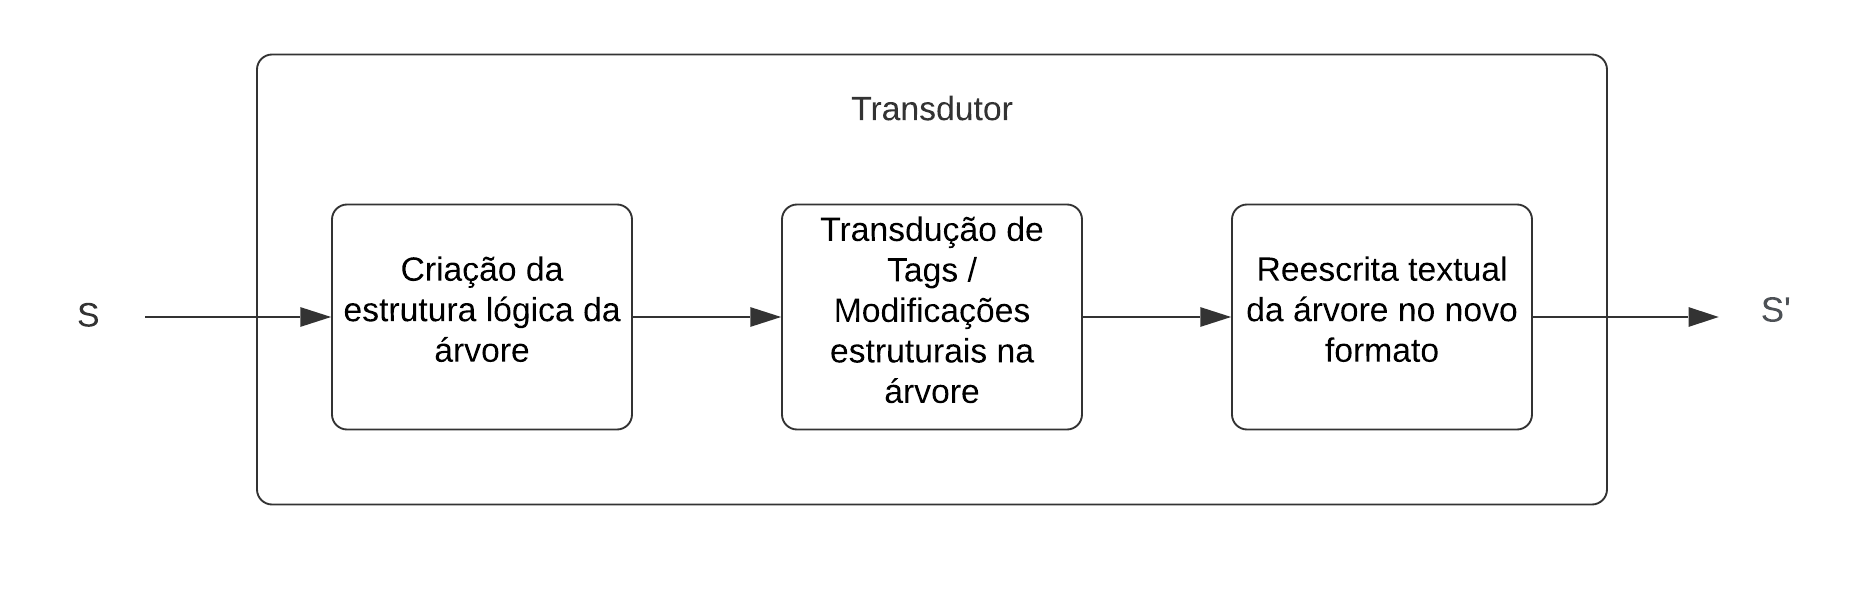
\includegraphics[width=\textwidth,scale=1.5]{imagens/fluxograma_transdutor.png}
    \caption[Fluxograma - transdutor]{Fluxograma descrevendo as etapas do transdutor}
    \label{fig:fluxograma_transdutor}
\end{figure}
\end{center}

O transdutor pode ser encontrado no GitHub do autor, \url{https://github.com/Fernandomn/como-treinar-seu-parser}.
